    %!xelatex = 'xelatex --halt-on-error %O %S'

\documentclass{thuemp}
\begin{document}

% 标题,作者
\emptitle{微波电子自旋共振与铁磁共振实验研究}
\empauthor{王驰}{王合英}

% 奇数页页眉
\fancyhead[CO]{{\footnotesize 王驰: 微波电子自旋共振与铁磁共振实验研究}}

%%%%%%%%%%%%%%%%%%%%%%%%%%%%%%%%%%%%%%%%%%%%%%%%%%%%%%%%%%%%%%%%
% 关键词 摘要 首页脚注
%%%%%%%%关键词
\Keyword{电子自旋共振,铁磁共振,微波技术,扫场,朗德$g$因子}
\twocolumn[
\begin{@twocolumnfalse}
\maketitle

%%%%%%%%摘要
\begin{empAbstract}

\end{empAbstract}

%%%%%%%%英文标题、作者、摘要、关键词
\emptitleEn{Electron Spin Resonance and Ferromagnetic Resonance Experiments}
\empauthorEn{Chi Wang}{Heying Wang}
\KeywordEn{Electron spin resonance, Ferromagnetic resonance, Microwave technology, Sweep field, Landé g-factor}

\begin{empAbstractEn}

\end{empAbstractEn}

%%%%%%%%首页角注
\empfirstfoot{2025-04-20}{2025-05-07}{2022012259}{chi-wang22@mails.tsinghua.edu.cn}
\end{@twocolumnfalse}
]
%%%%%%%%!首页角注可能与正文重叠,请通过调整正文中第一页的\enlargethispage{-3.3cm}位置手动校准正文底部位置:
%%%%%%%%%%%%%%%%%%%%%%%%%%%%%%%%%%%%%%%%%%%%%%%%%%%%%%%%%%%%%%%%
%  正文由此开始
\wuhao 
%  分栏开始

\section{引言}
\enlargethispage{-3.3cm}
\section{实验内容}

\subsection{电子自旋共振}

\subsubsection{电子自旋共振的描述}

当具有未成对电子的物质置于外加磁场中时,电子自旋会与磁场相互作用,导致能级分裂。能级分裂宽度$\Delta E$与外加磁场强度$B$以及电子磁矩$\mu$有关,满足关系式:

\begin{equation}
\Delta E = \mu B
\end{equation}

其中电子磁矩可以进一步用Bohr磁子$\mu_B = \frac{e\hbar}{2m_e}$和朗德$g$因子$g$表示为:

\begin{equation}
\mu = g \mu_B
\end{equation}

在电磁波作用下,当电磁波频率$\nu$与能级分裂频率相等时,电子自旋会发生共振跃迁,对电磁波的吸收达到极大,满足关系式:

\begin{equation}
h \nu  = \Delta E = g \mu_B B
\end{equation}

在电子由低能态跃迁至高能态后,通过与晶格以及周围电子的相互作用,系统回到低能态,伴随各向电磁波辐射,此过程称为弛豫。由于弛豫作用的存在,即使是在共振条件完全满足时,稳态下仍然会有一定数量的电子处于低能态,因此能在实验上测量到一稳定的共振吸收。

\subsubsection{测量系统与样品选择}

对于电子自旋共振,朗德$g$因子值接近于2;实验室中电磁铁一般可产生$0.1$\si{\tesla}~$1.0$\si\tesla 的磁场,对应于共振频率在数个\si{\giga\hertz},因而为测量电子自旋共振信号,需要使用微波波段电磁波源,以及波导、谐振腔等微波器件。

在本次实验中,我们使用北京大华DH1121A型3\si{\centi\meter}固态信号源作为微波源,配合BJ-100型波导管等微波器件,以及岩崎(IWATSU)SS-7802A型模拟示波器,对电子自旋共振和铁磁共振现象进行研究。如图【】所示,样品置于谐振腔内,通过一电磁铁提供磁场;微波源输出的微波信号通过隔离期、衰减器、环行器传输至反射式谐振腔,并在与样品相互作用后,再通过环行器以及波导管传输至晶体检波器

由于产生微波的元件本身频率调节有一定难度,在实验上通过常通过调节外加磁场,并观察微波功率吸收随之发生的变化,以吸收最大时对应的磁感应强度与微波源频率计算出朗德$g$因子。

在稳定存在的物质中,难以找到孤电子。历史上曾使用X射线照射小分子有机物,引起部分分子电离,进而得到含孤电子体系用于测量。在本次实验中,我们使用1,1-二苯基-2-(1,4,6-三硝基苯基)肼自由基(1,1-Diphenyl-2-picrylhydrazyl radical, DPPH)作为实验材料:DPPH本身是一种相对稳定的自由基,其分子中含有一个未成对电子(如图【】),能够产生较强的自旋共振信号。

在本部分测量中,DPPH样品被置于反射式谐振腔内,其几何尺寸可调,以适应于不同频率的微波信号。

在实验之初,需要选定适当微波源频率,并由此计算波导内波长$\lambda_g$,进而调整反射式谐振腔腔长,以及被测量样品的摆放位置。

所使用波导管为BJ-100型矩形波导,其宽度$a=22.86\pm0.07$ \si{\milli\meter},对应主模频率区间为$8.20 \approx 12.50$ \si{\giga\hertz}。

综合微波源以及波导管特性,选取微波源输出频率在$9$\si{\giga\hertz}附近,设定输出后借助直读式频率计读出$\nu  = 8.960 \pm 0.005$ \si{\giga\hertz},对应计算得到波长$\lambda$以及波导波长$\lambda_g$:

\begin{equation}
\lambda = \frac{c}{\nu} = 
\end{equation}

\begin{equation}
\lambda_g = \frac{\lambda}{\sqrt{1 - \left(\frac{\lambda}{2a}\right)^2}} = 
\end{equation}

在反射式谐振腔中,为使样品的自旋共振信号最大,应当使谐振腔内电磁场形成驻波,且样品应放置在腔内驻波磁感应强度幅值最大处。谐振腔长$L$,样品与谐振腔端面距离$d$和波导波长$\lambda_g$满足以下关系:

\begin{equation}
L = \frac{n}{2}\lambda_g \quad (n \in \mathbb{Z}^+)
\end{equation}

\begin{equation}
d = \frac{m}{2}\lambda_g \quad (m \in \mathbb{Z}^+)
\end{equation}

在本次实验中,选取谐振腔长$L=3\lambda_g\approx$,样品与谐振腔端面距离$d=\frac{3}{2}\lambda_g\approx$。为确认取到谐振腔内驻波磁感应强度幅值最大处,通过反复联合调节样品位置和谐振腔长度,观察,最终得到谐振腔内驻波磁感应强度幅值最大处的样品位置$d \approx 73.4 $\si{\milli\meter}。

\subsubsection{借助扫场信号观察电子自旋共振信号}

电子自旋共振频宽可能较窄,且晶体检波器-微安表系统对微波功率变化的响应较慢,因此在实验中借助磁共振实验仪的扫场功能,使用示波器确认共振发生所对应的中心频率:在一恒定励磁电流基础上,加一周期变化且幅值较小的周期信号,即“扫场信号”,由此样品电子自旋对磁感应强度变化的响应,会在时域上被展开成一个脉冲信号,显示在示波器上;调节励磁电流中心值$B$,直至这一脉冲信号中心落在示波器屏幕中心位置,此时$B_0$即满足样品电子自旋共振条件。

在本实验中,扫场信号为一锯齿波(如图【】),因而在一个扫描周期内,会在示波器上显示为两个脉冲信号:第一个脉冲信号对应于扫场信号上升段,第二个脉冲信号对应于扫场信号下降段。判定样品电子自旋共振条件时,实际取两脉冲信号中心值近似相等作为判据。

\subsection{铁磁共振}

\subsubsection{铁磁共振的描述}

在铁磁体中,电子自旋方向之间存在显著关联,在外加适当频率交变磁场时,会相类似地表现出自旋共振现象,整体宏观磁化矢量发生进动,并伴有对对应频率电磁波能量的强烈吸收。

在铁磁体系中,弛豫现象较之于电子自旋共振更为显著。为描述顺磁系统的宏观磁矩进动以及弛豫现象,通常使用Bloch方程描述宏观磁化矢量$\mathbf{M}$的时间演化:

\begin{equation}
\begin{aligned}
    \frac{\d M_x}{\d t} &= \gamma (\mathbf{M} \times \mathbf{B'})_x - \frac{M_x}{\tau_2} \\
    \frac{\d M_y}{\d t} &= \gamma (\mathbf{M} \times \mathbf{B'})_y - \frac{M_y}{\tau_2} \\
    \frac{\d M_z}{\d t} &= \gamma (\mathbf{M} \times \mathbf{B'})_z - \frac{M_z - M_z^0}{\tau_1}
\end{aligned}
\end{equation}

其中已选取坐标轴使得外加磁场$\mathbf{B}$沿$z$轴方向,$\mathbf{B'}$为外加的交变磁场$\tau_1$和$\tau_2$分别为纵向弛豫时间和横向弛豫时间,分别对应自旋-晶格相互作用和自旋-自旋相互作用。

类似于电子自旋共振,铁磁共振也会在外加磁感应强度满足特定条件时发生共振跃迁,伴随对对应频率电磁波能量的强烈吸收。对于铁磁物质,这一吸收作用还可以通过交变磁场下整体复磁导率$\tilde\mu $来描述:

\begin{equation}
    \tilde\mu = \mu' + i\mu''
\end{equation}

其中$\mu'$对应于其在稳定磁场下的磁导率,$\mu''$对应于交变磁能在铁磁体中耗散的部分。调整外加磁感应强度至发生铁磁共振时,$\omega = \frac{g}{\mu_B\hbar} B_0$,$\mu''$也会达到极大值,且存在一共振展宽$\Delta B$对应于铁磁共振的频宽。在本实验中,我们定义$\mu'' = \frac 1 2 \mu''_{\mathrm{max}}$时对应的磁感应强度间隔$(B_1 - B_2)$作为$\Delta B$。

在一般情况下,$\tau_1 = \tau_2 \approx 2/\gamma \Delta B$;方便起见将$\tau_1, \tau_2$统称为弛豫时间$\tau$,则有:

\begin{equation}
    \tau = \frac{2}{\gamma\Delta B} = \frac{4\pi}{\nu}\frac{B_0}{\Delta B}
\end{equation}



\subsubsection{测量系统与样品选择}

在铁磁共振实验中,我们将使用传输式谐振腔,对多晶铁氧体样品的铁磁共振进行测量。如图【】,微波源产生的微波信号经过隔离器、衰减器等微波器件进入传输式谐振腔,并在与样品作用后进入下一段波导,进而通过其中的晶体检波器以及与之相连的检流计,读出透射微波功率。在本次测量中,我们将假定检波二极管工作在信号电流与场强平方成正比的区间,此时读出的电流即正比于功率。

\section{实验结果与分析}

\subsection{电子自旋共振朗德$g$因子计算}

调节励磁电流中心值以及扫场幅度,观察到励磁电流为$I_{m,0} = 1.821$\si\ampere 时,示波器上显示的两个脉冲信号中心位置相近,且幅值均较大。结合实验所使用电磁体特性:

\begin{equation}
    B = 0.0152 ~\text{\si\tesla} + 0.1632 ~\text{\si\tesla / \si\ampere} \cdot I_m
\end{equation}

得到此时样品电子自旋共振条件下的磁感应强度为$B_0 = 0.3123$ \si\tesla。给出$g$因子测量值:

\begin{equation}
g = \frac{h \nu}{\mu_B B_0} = \frac{4\pi m_e}{e} \frac{\nu}{B_0}\approx 2.049
\end{equation}

测量结果与公认的电子$g$因子已经相当接近。

\subsection{铁磁共振朗德$g$因子计算}

在此部分实验中,设定频率为$\nu = 9.029 \pm 0.005~\text{\si{\giga \hertz}}$为确定透射功率取最小值,以及透射功率恰好取到$P_{1/2}$时的外加磁场,对测量得到的功率-磁场关系,通过使用适当函数进行拟合,确定吸收峰中心值,并反解得到$B_1, B_2$,进而利用【】式计算得到$\Delta B$。

选用Lorentz线型作为信号形状进行拟合,结果如下:

\begin{figure}[H]
    \centering
    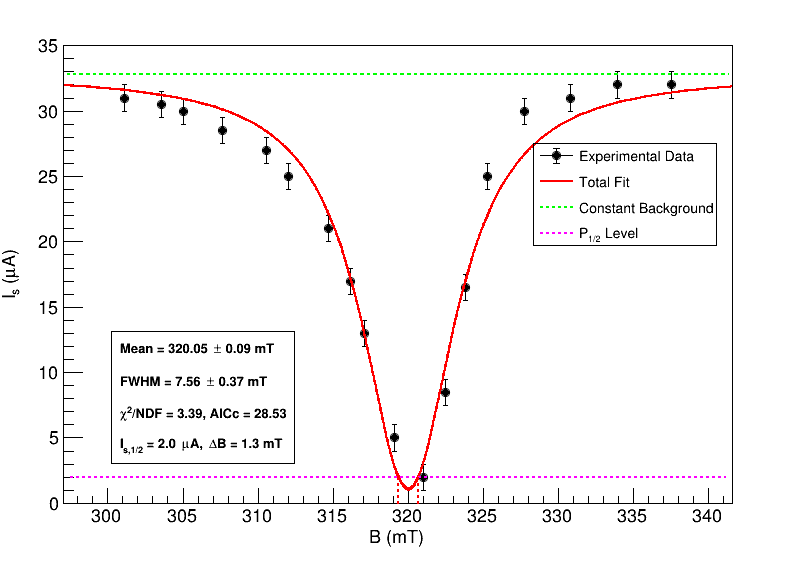
\includegraphics[width=0.9\linewidth]{../Data/FMR_ConstantBg_LorentzPeak.png}
    \caption{铁磁共振透射功率与外加磁场关系图} \label{fig:gmr_gradient}
\end{figure}

拟合得到参数如下:

\begin{table}[H]
    \centering
    \captionnamefont{\wuhao\bf\heiti}
    \captiontitlefont{\wuhao\bf\heiti}
    \caption{铁磁共振信号拟合结果} \label{tab:FMR_fit}
    \liuhao
    \begin{tabular}{cccc}
        \toprule
        中心值 & 半高全宽(FWHM) & 信号幅度 & 背景信号高度 \\
        $B_0/\text{\si\tesla}$ & $\Gamma_B/\text{\si\tesla}$ & $A/\text{\si{\micro\ampere}}$ & $I_{S,0}$\\
        \midrule
        0.32 & 7.5 & 31.8 & 32.8 \\
        \bottomrule
    \end{tabular}
\end{table}

此时可以根据共振峰中心值$B_0$求出$g$因子:

\begin{equation}
g = \frac{h \nu}{\mu_B B_0} = \frac{4\pi m_e}{e} \frac{\nu}{B_0}\approx 2.016
\end{equation}

如此得到的结果与自由电子$g$因子接近。

\subsection{铁磁共振弛豫时间分析}

根据表格\ref{tab:FMR_fit}进一步求出与$P_r, P_0, P_{1/2}$分别对应的信号电流值$I_r, I_0, I_{1/2}$,反解得到$B_{1}, B_{2}$:

\begin{table}[H]
    \centering
    \captionnamefont{\wuhao\bf\heiti}
    \captiontitlefont{\wuhao\bf\heiti}
    \caption{铁磁共振弛豫时间分析结果表} \label{tab:FMR_relax}
    \liuhao
    \begin{tabular}{cccccc}
        \toprule
        无吸收时 & 共振情形 & $\mu''$半宽 &
            \multicolumn{2}{c}{$\mu''$半宽所对应}\\
        信号电流 & 信号电流 & 信号电流     &  
            \multicolumn{2}{c}{外加磁场}\\
        $I_{0}/\text{\si{\micro\ampere}}$ & 
            $I_{r}/\text{\si{\micro\ampere}}$ &
            $I_{1/2}/\text{\si{\micro\ampere}}$&
            $B_1/\text{\si{\milli\tesla}}$ &
            $B_2/\text{\si{\milli\tesla}}$ \\ 
        \midrule
        32.80& 1.02 & 1.98 & 319.4 & 320.7 \\
        \bottomrule
    \end{tabular}
\end{table}

其中,根据检波二极管特性$I \propto E^2 \propto P$,使用以下关系式:

\begin{equation}
    I_{1/2} = \frac{2P_0P_r}{P_0+P_r}
\end{equation}

由以上结果,计算得:
\begin{equation}
    \Delta B = |B_1 - B_2| = 1.7 ~\text{\si{\milli\tesla}}
\end{equation}

\begin{equation}
    \tau = \frac{2}{\gamma\Delta B}
         = \frac{4\pi}{\nu}\frac{B_0}{\Delta B}
         \approx 262 ~ \text{ns}
\end{equation}

\section{结论}



%%%%%%%%%%%%%%%%%%%%%%%%%%%%%%%%%%%%%%%%%%%%%%%%%%%%%%%%%%%%%%%%
%  参考文献
%%%%%%%%%%%%%%%%%%%%%%%%%%%%%%%%%%%%%%%%%%%%%%%%%%%%%%%%%%%%%%%%
\renewcommand\refname{\heiti\wuhao\centerline{参考文献}\global\def\refname{参考文献}}
\vskip 12pt

\let\OLDthebibliography\thebibliography
\renewcommand\thebibliography[1]{
  \OLDthebibliography{#1}
  \setlength{\parskip}{0pt}
  \setlength{\itemsep}{0pt plus 0.3ex}
}

{
\renewcommand{\baselinestretch}{0.9}
\liuhao
\bibliographystyle{gbt7714-numerical}
\bibliography{./Report/TempExample}
}
\newpage
\appendix

\section{铁磁共振信号拟合函数的选择}

对铁磁共振信号,在拟合过程中曾先后使用高斯型、洛伦兹型和水晶球函数作为信号函数。其中,水晶球函数表达式为:


以上各组合拟合结果如下:


其中,水晶球函数虽然拟合描述最好,但是总共使用6个拟合参数,数量过多,存在潜在的过拟合风险。结合曲线符合程度,选择使用洛伦兹型峰描述共振信号。



\section{源代码获取}

本实验所使用的代码,包括本篇报告的\LaTeX 源码,均可从\url{github.com/Eric100911/mpl-ESR-FMR}下载。

\end{document}